\documentclass[10pt,a4paper]{article}
\usepackage[margin=21mm,headheight=15pt]{geometry}
\usepackage[T1]{fontenc}
\usepackage{lmodern,amsmath,amssymb,tikz,graphicx,hyperref,fancyhdr,enumitem,needspace}
\usetikzlibrary{arrows.meta,positioning,calc,decorations.pathmorphing}
\definecolor{ink}{RGB}{20,53,78}
\hypersetup{colorlinks=true,urlcolor=ink,linkcolor=ink}
\setlength{\parindent}{0pt}\setlength{\parskip}{5pt}
\emergencystretch=3em
\pagestyle{fancy}\fancyhf{}\fancyfoot[C]{\thepage}
\renewcommand{\headrulewidth}{.3pt}
\newcommand{\task}[2]{\par\medskip{\color{ink}\Large\bfseries #1. #2}\par\smallskip}
\newcommand{\answer}{\par\smallskip\textbf{Worked reasoning.} }
\setlist[enumerate]{label=\textbf{(\alph*)},leftmargin=7mm,itemsep=7pt}
\begin{document}
\fancyhead[L]{\small Control of Dynamical Systems}
\fancyhead[R]{\small Integrated design studies}
{\color{ink}\LARGE\bfseries Integrated design studies}\par
{\large From a physical model to a defensible design decision}\par
\textbf{Worked solutions -- five integrated problems}\par
{\small\textbf{Evidence boundary.} Original hypothetical scenarios. Derive, calculate and justify decisions; every numerical record is synthetic. Figures are conceptual and not to scale.}
\task{1}{Interacting water tanks: from flow laws to a feasible controller}
Two open tanks have constant areas $A_1=0.02$ m$^2$ and $A_2=0.03$ m$^2$. Their submerged connection obeys
\[
q_{12}=k_{12}\operatorname{sgn}(h_1-h_2)\sqrt{|h_1-h_2|},\qquad
q_2=k_2\sqrt{h_2},
\]
where $k_{12}=0.004$ and $k_2=0.003$ m$^{5/2}$/s. The pump feeds only tank 1. Nominal inflow is $\bar q=0.0012$ m$^3$/s; the measured output is $h_2$. Areas and discharge coefficients are hypothetical. Assume nonnegative levels, no overflow and ideal sensing.
\begin{center}\resizebox{\ifdim\width>.98\linewidth.98\linewidth\else\width\fi}{!}{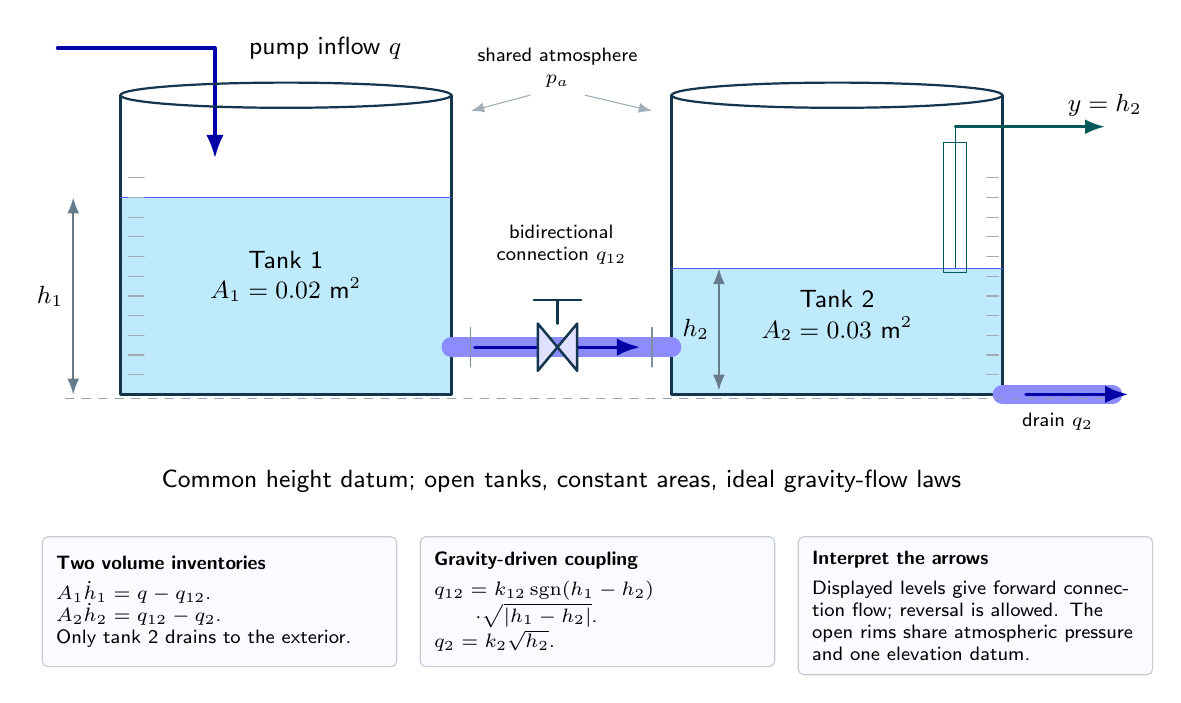
\begin{tikzpicture}[
font=\sffamily\small,>=Latex,line cap=round,line join=round,
wall/.style={draw=ink,line width=1.2pt,fill=blue!5},
water/.style={fill=cyan!25,draw=none},
metal/.style={draw=ink,fill=blue!12,line width=.9pt},
flow/.style={->,draw=blue!65!black,line width=1.2pt},
heat/.style={->,draw=orange!85!black,line width=1.1pt},
measure/.style={->,draw=teal!70!black,line width=.9pt},
dim/.style={<->,draw=ink!65,line width=.6pt},
spring/.style={draw=ink,decorate,decoration={coil,aspect=.5,segment length=4pt,amplitude=3pt}},
wire/.style={draw=ink,line width=1pt},
lab/.style={align=center,font=\sffamily\small},
smalllab/.style={align=center,font=\sffamily\scriptsize}]

\fill[water](1,1)rectangle(5.2,3.5);
\fill[water](8,1)rectangle(12.2,2.6);
\draw[wall,fill=none](1,4.8)--(1,1)--(5.2,1)--(5.2,4.8);
\draw[wall,fill=none](8,4.8)--(8,1)--(12.2,1)--(12.2,4.8);
\draw[blue!65](1,3.5)--(5.2,3.5)(8,2.6)--(12.2,2.6);
\draw[blue!45,line width=7pt](5.2,1.6)--(8,1.6);
\draw[blue!45,line width=7pt](12.2,1)--(13.6,1);
\draw[flow](5.5,1.6)--(7.6,1.6);
\draw[flow](12.5,1)--(13.8,1);
\draw[metal](6.3,1.3)--(6.8,1.9)--(6.8,1.3)--(6.3,1.9)--cycle;
\draw[wire](6.55,1.9)--(6.55,2.2)(6.25,2.2)--(6.85,2.2);
\node[smalllab]at(6.6,2.9){bidirectional\\connection $q_{12}$};
\node[smalllab]at(12.9,.65){drain $q_2$};
\draw[flow](.2,5.4)--(2.2,5.4)--(2.2,4);
\node[lab]at(3.6,5.4){pump inflow $q$};
\node[lab]at(3.1,2.5){Tank 1\\$A_1=0.02$ m$^2$};
\node[lab]at(10.1,2){Tank 2\\$A_2=0.03$ m$^2$};
\draw[dim](.4,1)--node[left]{$h_1$}(.4,3.5);
\draw[dim](8.6,1.05)--node[left]{$h_2$}(8.6,2.6);
\draw[teal!70!black](11.6,2.6)--(11.6,4.4);
\draw[measure](11.6,4.4)--(13.5,4.4)node[above]{$y=h_2$};
\draw[ink!45,dashed](.3,.95)--(13.5,.95);
\node[lab]at(6.6,-.1){Common height datum; open tanks, constant areas, ideal gravity-flow laws};
% REFINED EQUIPMENT DETAILS

% Open tank rims, submerged ports and an instrument associated with h2.
\draw[ink,line width=.8pt](3.1,4.8)ellipse(2.1 and .16);
\draw[ink,line width=.8pt](10.1,4.8)ellipse(2.1 and .16);
\foreach \x in {5.45,7.75}{\draw[ink!55](\x,1.35)--(\x,1.85);}
\draw[teal!70!black](11.45,2.55)rectangle(11.75,4.2);
\foreach \y in {1.25,1.5,...,3.75}{\draw[ink!40](1.1,\y)--(1.3,\y)(12,\y)--(12.15,\y);}
\node[smalllab]at(6.55,5.15){shared atmosphere\\$p_a$};
\draw[ink!40,->](6.2,4.8)--(5.45,4.6);\draw[ink!40,->](6.9,4.8)--(7.75,4.6);

\node[draw=ink!25,fill=blue!2,rounded corners=2pt,anchor=north west,text width=4.15cm,minimum height=1.65cm,inner sep=5pt,align=left,font=\sffamily\scriptsize]at(0.0,-0.8){\textbf{Two volume inventories}\\[3pt]$A_1\dot h_1=q-q_{12}$.\\$A_2\dot h_2=q_{12}-q_2$.\\Only tank 2 drains to the exterior.};
\node[draw=ink!25,fill=blue!2,rounded corners=2pt,anchor=north west,text width=4.15cm,minimum height=1.65cm,inner sep=5pt,align=left,font=\sffamily\scriptsize]at(4.8,-0.8){\textbf{Gravity-driven coupling}\\[3pt]$q_{12}=k_{12}\operatorname{sgn}(h_1-h_2)$\\$\qquad\cdot\sqrt{|h_1-h_2|}$.\\$q_2=k_2\sqrt{h_2}$.};
\node[draw=ink!25,fill=blue!2,rounded corners=2pt,anchor=north west,text width=4.15cm,minimum height=1.65cm,inner sep=5pt,align=left,font=\sffamily\scriptsize]at(9.6,-0.8){\textbf{Interpret the arrows}\\[3pt]Displayed levels give forward connection flow; reversal is allowed. The open rims share atmospheric pressure and one elevation datum.};
\end{tikzpicture}
}\par{\small Interacting tanks share a submerged connection at a common datum. Flow reverses if the level ordering reverses. Only tank 2 drains to the exterior; this is not a cascade with a freely falling inter-tank stream.}\end{center}
\begin{enumerate}
\Needspace{7\baselineskip}\item Starting from conservation of volume, derive the nonlinear state equations. Find both equilibrium heights and explain why the connection flow depends on a level difference.
\answer For each constant-area vessel, stored volume is $A_i h_i$. The balances are
\[
A_1\dot h_1=q-q_{12},\qquad A_2\dot h_2=q_{12}-q_2.
\]
At equilibrium both outlet flows equal $\bar q$. Thus $\bar h_2=(\bar q/k_2)^2=0.16$ m and $\bar h_1-\bar h_2=(\bar q/k_{12})^2=0.09$ m, so $\bar h_1=0.25$ m. A submerged connection responds to the hydrostatic pressure difference, not the first tank's height alone. The sign convention permits reversal when the second level exceeds the first.
\Needspace{7\baselineskip}\item Linearize about that equilibrium using deviation variables. Derive the transfer function from inflow to the second level, its poles and its DC gain. State where the linearization ceases to be differentiable.
\answer The local flow slopes are $g_{12}=k_{12}/(2\sqrt{0.09})=1/150$ m$^2$/s and $g_2=k_2/(2\sqrt{0.16})=0.00375$ m$^2$/s. Consequently
\[
\delta\dot h=\begin{bmatrix}-1/3&1/3\\2/9&-25/72\end{bmatrix}\delta h+
\begin{bmatrix}50\\0\end{bmatrix}\delta q,\quad
\delta y=[0\quad1]\delta h.
\]
Eliminating the first state yields $G(s)=(100/9)/(s^2+49s/72+1/24)$. Its poles are approximately $-0.612532,-0.0680237$ s$^{-1}$ and its DC gain is $800/3$ s/m$^2$. These finite derivatives require strictly positive $h_2$ and nonzero level difference; the ideal square-root laws are not differentiable at an empty outlet or equal tank levels.
\Needspace{7\baselineskip}\item Increase the constant inflow by $10^{-4}$ m$^3$/s. Compare the linear and exact equilibrium changes of $h_2$, expressing the error relative to the exact change. Explain why a small input increment is not a universal accuracy certificate.
\answer The linear prediction is $\delta h_2=G(0)\delta q=(800/3)10^{-4}=0.0266667$ m. The exact new level is $(0.0013/0.003)^2=0.1877778$ m, so the actual change is $0.0277778$ m. The prediction underestimates this change by $0.0011111$ m, or 4 percent. The relative error of the total height would be a different metric. This comparison checks one steady perturbation; transient error, other operating points and approach to empty/equal-level singularities require separate analysis.
\Needspace{7\baselineskip}\item Use deviation PI control $\delta q=k_p(r-\delta h_2)+k_i\int(r-\delta h_2)\,dt$. Derive the characteristic polynomial and the strict stability region for positive gains. Check $k_p=0.001$ m$^2$/s and $k_i=0.0001$ m$^2$/s$^2$.
\answer Write $a_1=49/72$, $a_0=1/24$ and $b=100/9$. Then $1+(k_p+k_i/s)G=0$ gives
\[
p(s)=s^3+a_1s^2+(a_0+bk_p)s+bk_i.
\]
The cubic Routh first column is $1,a_1,[a_1(a_0+bk_p)-bk_i]/a_1,bk_i$. For $k_p,k_i>0$, strict stability therefore requires $k_i<a_1(a_0+bk_p)/b$. The selected gains give $a_0+bk_p=0.0527778$ and $bk_i=0.00111111$, with $a_1(a_0+bk_p)\approx0.0359182>0.00111111$. The poles are about $-0.594991$ and $-0.0427825\pm0.00609126j$. This is a local unsaturated result.
\Needspace{7\baselineskip}\item The pump is limited to $0\le q\le0.0015$ m$^3$/s. Can the second level be held at 0.30 m? Determine the highest feasible equilibrium level and describe the implication for integral action.
\answer At any equilibrium $q=k_2\sqrt{h_2}$. A 0.30 m target needs $q=0.003\sqrt{0.30}\approx0.00164317$ m$^3$/s, exceeding the limit. The largest equilibrium second level is $(0.0015/0.003)^2=0.25$ m, with $h_1=0.25+(0.0015/0.004)^2=0.390625$ m if tank height permits. A persistent positive error can wind up an unconstrained integrator. Anti-windup can limit controller-state accumulation but cannot supply missing pump capacity or prevent overflow omitted from the model.
\Needspace{7\baselineskip}\item Propose a simulation and identification protocol that could falsify the local model. Include initial conditions, reverse connection flow, numerical convergence and the distinction between simulation and physical validation.
\answer Integrate the nonlinear balances and local deviation model from the same nominal initial state, then compare several positive and negative inflow steps with levels and volumes reported in SI units. Repeat from perturbed states, including $h_2>h_1$, using the signed connection law. Guard against negative levels and stop at overflow rather than extrapolating beyond the model. Tighten solver tolerances and compare volume balance residuals. For identification, use separate excitation and validation records; do not fit and score on the same response. These are synthetic model tests. Physical validation additionally requires calibrated level/flow sensors, documented apparatus and measured records, none of which are supplied here.
\end{enumerate}

\newpage
\task{2}{Optical isolation with conflicting stiffness and travel requirements}
A hypothetical optical bench of mass $m=8$ kg sits on a parallel spring and viscous damper, with total stiffness $k=3200$ N/m and damping ratio $\zeta=0.08$. The floor displacement is $z(t)$ and payload displacement is $x(t)$, measured about static equilibrium. The floor can oscillate at 40 rad/s with amplitude 0.5 mm. The design brief asks for less payload motion than floor motion, static sag at most 3 mm and relative travel amplitude at most 0.6 mm.
\begin{center}\resizebox{\ifdim\width>.98\linewidth.98\linewidth\else\width\fi}{!}{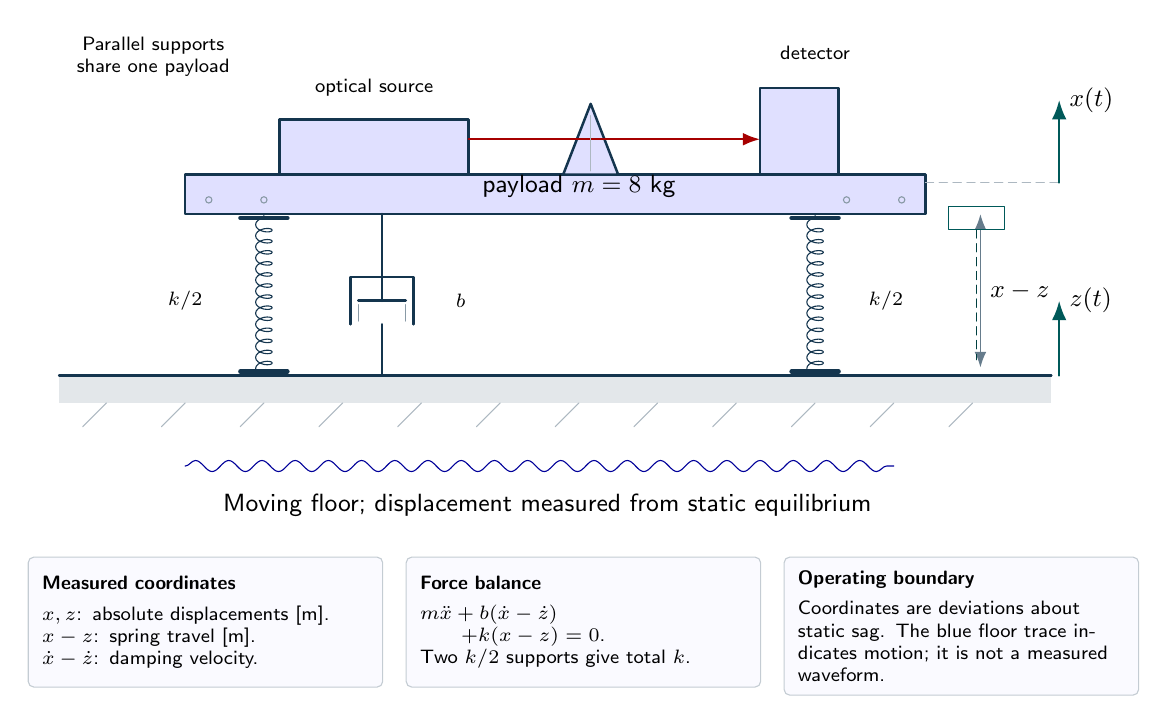
\begin{tikzpicture}[
font=\sffamily\small,>=Latex,line cap=round,line join=round,
wall/.style={draw=ink,line width=1.2pt,fill=blue!5},
water/.style={fill=cyan!25,draw=none},
metal/.style={draw=ink,fill=blue!12,line width=.9pt},
flow/.style={->,draw=blue!65!black,line width=1.2pt},
heat/.style={->,draw=orange!85!black,line width=1.1pt},
measure/.style={->,draw=teal!70!black,line width=.9pt},
dim/.style={<->,draw=ink!65,line width=.6pt},
spring/.style={draw=ink,decorate,decoration={coil,aspect=.5,segment length=4pt,amplitude=3pt}},
wire/.style={draw=ink,line width=1pt},
lab/.style={align=center,font=\sffamily\small},
smalllab/.style={align=center,font=\sffamily\scriptsize}]

\fill[ink!12](.4,.2)rectangle(13,.55);
\draw[ink,line width=1pt](.4,.55)--(13,.55);
\foreach \x in {1,2,...,12}{\draw[ink!35](\x,.2)--++(-.3,-.3);}
\draw[metal](2,2.6)rectangle(11.4,3.1);
\draw[spring](3,.55)--(3,2.6);
\draw[spring](10,.55)--(10,2.6);
\draw[wire](4.5,.55)--(4.5,1.2)(4.1,1.2)--(4.1,1.8)--(4.9,1.8)--(4.9,1.2);
\draw[wire](4.5,2.6)--(4.5,1.5)(4.2,1.5)--(4.8,1.5);
\draw[metal](3.2,3.1)rectangle(5.6,3.8);
\draw[metal](6.8,3.1)--(7.15,4)--(7.5,3.1)--cycle;
\draw[metal](9.3,3.1)rectangle(10.3,4.2);
\draw[red!65!black,->,line width=.7pt](5.6,3.55)--(9.3,3.55);
\node[smalllab]at(4.4,4.2){optical source};
\node[smalllab]at(10,4.65){detector};
\node[lab]at(7,2.95){payload $m=8$ kg};
\node[smalllab]at(2,1.5){$k/2$};\node[smalllab]at(10.9,1.5){$k/2$};
\node[smalllab]at(5.5,1.5){$b$};
\draw[dim](12.1,.65)--node[right]{$x-z$}(12.1,2.6);
\draw[ink!35,densely dashed](11.4,3)--(13.1,3);
\draw[measure](13.1,3)--(13.1,4.05)node[right]{$x(t)$};
\draw[measure](13.1,.55)--(13.1,1.5)node[right]{$z(t)$};
\draw[blue!60!black,decorate,decoration={snake,amplitude=2pt,segment length=12pt}](2,-.6)--(11,-.6);
\node[lab]at(6.6,-1.1){Moving floor; displacement measured from static equilibrium};
% REFINED EQUIPMENT DETAILS

% Fasteners, spring seats and a clearly resolved dashpot piston.
\foreach \x in {2.3,3,10.4,11.1}{\draw[ink!50](\x,2.78)circle(.04);}
\foreach \x in {3,10}{\draw[ink,line width=1.5pt](\x-.3,.6)--(\x+.3,.6)(\x-.3,2.55)--(\x+.3,2.55);}
\draw[ink!50](4.2,1.24)--(4.2,1.45)(4.8,1.24)--(4.8,1.45);
\draw[ink!35](7.15,3.15)--(7.15,3.85);
\draw[teal!70!black](11.7,2.4)rectangle(12.4,2.7);
\draw[teal!50!black,densely dashed](12.05,2.4)--(12.05,.75);
\node[smalllab,anchor=west]at(.5,4.6){Parallel supports\\share one payload};

\node[draw=ink!25,fill=blue!2,rounded corners=2pt,anchor=north west,text width=4.15cm,minimum height=1.65cm,inner sep=5pt,align=left,font=\sffamily\scriptsize]at(0.0,-1.75){\textbf{Measured coordinates}\\[3pt]$x,z$: absolute displacements [m].\\$x-z$: spring travel [m].\\$\dot x-\dot z$: damping velocity.};
\node[draw=ink!25,fill=blue!2,rounded corners=2pt,anchor=north west,text width=4.15cm,minimum height=1.65cm,inner sep=5pt,align=left,font=\sffamily\scriptsize]at(4.8,-1.75){\textbf{Force balance}\\[3pt]$m\ddot x+b(\dot x-\dot z)$\\$\qquad+k(x-z)=0$.\\Two $k/2$ supports give total $k$.};
\node[draw=ink!25,fill=blue!2,rounded corners=2pt,anchor=north west,text width=4.15cm,minimum height=1.65cm,inner sep=5pt,align=left,font=\sffamily\scriptsize]at(9.6,-1.75){\textbf{Operating boundary}\\[3pt]Coordinates are deviations about static sag. The blue floor trace indicates motion; it is not a measured waveform.};
\end{tikzpicture}
}\par{\small An optical payload rests on parallel spring and damping elements. The two springs each have stiffness $k/2$, giving total $k$. Both the floor and payload move; spring extension and damping velocity are relative quantities. Weight is balanced at the static equilibrium about which the model is written.}\end{center}
\begin{enumerate}
\Needspace{7\baselineskip}\item Draw the force balance and derive both $X/Z$ and $(X-Z)/Z$. Compute the natural frequency and damper coefficient; explain why replacing floor motion by an applied force changes the numerator.
\answer The spring and damper exert $-k(x-z)-b(\dot x-\dot z)$, so $m\ddot x+b(\dot x-\dot z)+k(x-z)=0$. Therefore
\[
\frac{X}{Z}=\frac{bs+k}{ms^2+bs+k},\qquad
\frac{X-Z}{Z}=\frac{-ms^2}{ms^2+bs+k}.
\]
Here $\omega_n=\sqrt{k/m}=20$ rad/s and $b=2\zeta\sqrt{mk}=25.6$ N s/m. A force applied to a fixed-base mass instead gives $X/F=1/(ms^2+bs+k)$, with different units and numerator. Confusing the two inputs changes both resonance and high-frequency predictions.
\Needspace{7\baselineskip}\item Evaluate absolute displacement and relative travel at the stated excitation. Check the two dynamic requirements separately.
\answer For $r=\omega/\omega_n=2$,
\[
|X/Z|=\frac{\sqrt{1+(2\zeta r)^2}}{\sqrt{(1-r^2)^2+(2\zeta r)^2}}\approx0.34801,
\quad |(X-Z)/Z|=\frac{r^2}{\sqrt{(1-r^2)^2+(2\zeta r)^2}}\approx1.32581.
\]
Payload amplitude is approximately 0.1740 mm, below the floor amplitude, so the isolation requirement is met. Relative travel is approximately 0.66291 mm, exceeding 0.6 mm. Small absolute motion does not imply small spring travel.
\Needspace{7\baselineskip}\item Show that displacement isolation occurs only above $\sqrt2\,\omega_n$, independently of positive damping. Combine this with the sag requirement to decide whether any passive linear spring can satisfy both specifications at 40 rad/s.
\answer Squaring $|X/Z|<1$ cancels the damping terms and gives $1<(1-r^2)^2$, hence $r>\sqrt2$ for positive frequency. Isolation at 40 rad/s requires $\omega_n<40/\sqrt2=28.2843$ rad/s. Meanwhile sag is $mg/k=g/\omega_n^2$, so sag at most 0.003 m requires $\omega_n\ge\sqrt{9.81/0.003}=57.1839$ rad/s. The intervals do not overlap. Changing mass alone cannot repair this contradiction because both constraints depend on $k/m$. A different support architecture or relaxed specification is required.
\Needspace{7\baselineskip}\item Would raising the damping ratio to 0.4 cure the travel issue without a cost? Calculate the two amplitudes at 40 rad/s and compare resonance and high-frequency behavior.
\answer With $\zeta=0.4$ and $r=2$, absolute transmissibility is $\sqrt{3.56}/\sqrt{11.56}\approx0.55494$ and relative transmissibility is $4/\sqrt{11.56}\approx1.17647$. The amplitudes are approximately 0.2775 and 0.5882 mm. Travel now meets 0.6 mm, but isolation is weaker. At $r=1$, absolute transmissibility falls from $\sqrt{1+0.16^2}/0.16\approx6.3295$ to $\sqrt{1+0.8^2}/0.8\approx1.6008$. At high frequency the viscous transmission scales as $2\zeta/r$; larger damping improves resonance while increasing this asymptotic transmission. It does not solve the sag conflict.
\Needspace{7\baselineskip}\item Derive an energy balance valid for a moving base. Explain why energy need not decrease even when the damper is passive.
\answer Use $E=\tfrac12m\dot x^2+\tfrac12k(x-z)^2$. Differentiation and the equation of motion give
\[
\dot E=-b(\dot x-\dot z)^2-
[b(\dot x-\dot z)+k(x-z)]\dot z.
\]
The first term is irreversible viscous dissipation. The second is boundary work done through floor motion and can have either sign. Setting $\dot z=0$ recovers nonincreasing energy, but applying that fixed-base conclusion to a moving foundation would omit the excitation power.
\Needspace{7\baselineskip}\item Write a justified design decision and a minimum validation plan, including what can and cannot be inferred from a simulated frequency-response curve.
\answer Reject the combined stiffness brief as infeasible for this passive linear architecture. If sag is relaxed, the larger damping choice meets the specified travel amplitude at 40 rad/s at the cost of weaker isolation there; it still needs checks over the full disturbance spectrum. Validate the transfer functions against time-domain sinusoidal integration after transients decay, sweep payload mass and damping, and check relative travel explicitly. Finite travel, nonlinear mounts, dry friction and structural modes remain outside the model. A synthetic Bode curve verifies a mathematical prediction; it does not demonstrate actual vibration performance.
\end{enumerate}

\newpage
\task{3}{A motor speed servo under voltage and load constraints}
A hypothetical DC motor has $R=2\,\Omega$, $L=0.02$ H, $J=0.01$ kg m$^2$, $b=0.02$ N m s/rad, $k_t=0.1$ N m/A and $k_e=0.1$ V s/rad. The load torque is 0.03 N m. The requested speed is 5 rad/s and the voltage limit is $|V|\le2$ V. Positive torque and speed use the same orientation.
\begin{center}\resizebox{\ifdim\width>.98\linewidth.98\linewidth\else\width\fi}{!}{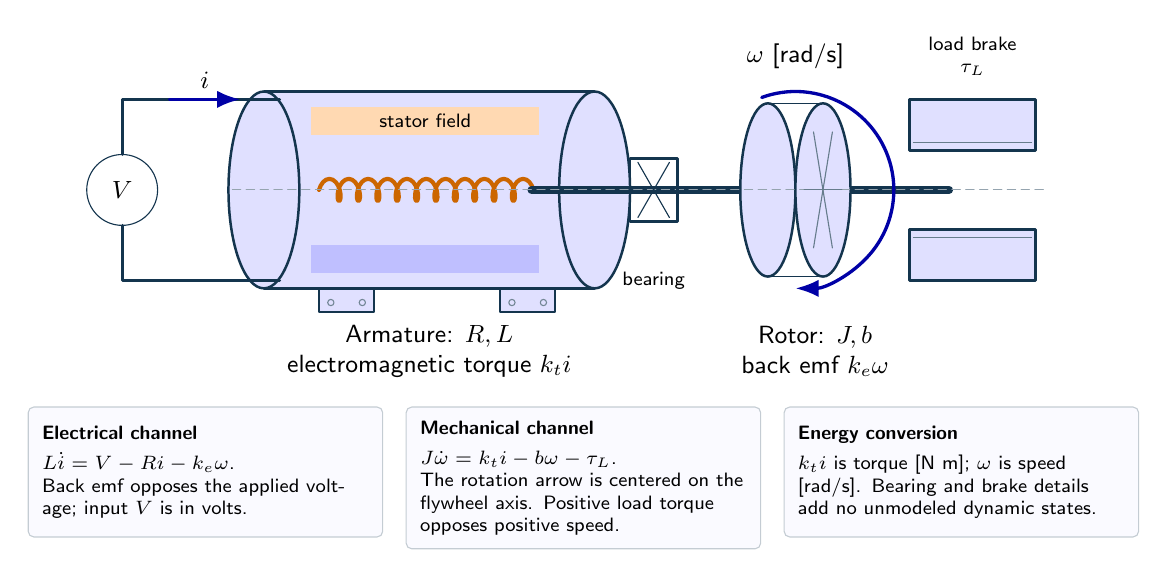
\begin{tikzpicture}[
font=\sffamily\small,>=Latex,line cap=round,line join=round,
wall/.style={draw=ink,line width=1.2pt,fill=blue!5},
water/.style={fill=cyan!25,draw=none},
metal/.style={draw=ink,fill=blue!12,line width=.9pt},
flow/.style={->,draw=blue!65!black,line width=1.2pt},
heat/.style={->,draw=orange!85!black,line width=1.1pt},
measure/.style={->,draw=teal!70!black,line width=.9pt},
dim/.style={<->,draw=ink!65,line width=.6pt},
spring/.style={draw=ink,decorate,decoration={coil,aspect=.5,segment length=4pt,amplitude=3pt}},
wire/.style={draw=ink,line width=1pt},
lab/.style={align=center,font=\sffamily\small},
smalllab/.style={align=center,font=\sffamily\scriptsize}]

\draw[metal](3,1.4)rectangle(7.2,3.9);
\draw[metal](3,2.65)ellipse(.45 and 1.25);
\draw[metal](7.2,2.65)ellipse(.45 and 1.25);
\fill[orange!30](3.6,3.35)rectangle(6.5,3.7);
\fill[blue!25](3.6,1.6)rectangle(6.5,1.95);
\node[smalllab]at(5.05,3.53){stator field};
\draw[orange!80!black,line width=1.5pt,decorate,decoration={coil,segment length=7pt,amplitude=4pt}](3.7,2.65)--(6.5,2.65);
\draw[ink,line width=3pt](6.4,2.65)--(11.7,2.65);
\draw[metal](9.4,2.65)ellipse(.35 and 1.1);
\draw[metal](10.1,2.65)ellipse(.35 and 1.1);
\draw[ink](9.4,3.75)--(10.1,3.75)(9.4,1.55)--(10.1,1.55);
\draw[metal](11.2,1.5)rectangle(12.8,2.15);
\draw[metal](11.2,3.15)rectangle(12.8,3.8);
\node[smalllab]at(12,4.35){load brake\\$\tau_L$};
\draw[flow]($(9.75,2.65)+(110:1.25)$)arc[start angle=110,end angle=-90,radius=1.25];
\node[lab]at(9.75,4.35){$\omega$ [rad/s]};
\draw[wire](3.2,3.8)--(1.2,3.8)--(1.2,3.1)(3.2,1.5)--(1.2,1.5)--(1.2,2.2);
\draw[ink](1.2,2.65)circle(.45);
\node at(1.2,2.65){$V$};
\draw[flow](1.8,3.8)--(2.7,3.8)node[midway,above]{$i$};
\node[lab]at(5.1,.6){Armature: $R,L$\\electromagnetic torque $k_t i$};
\node[lab]at(10,.6){Rotor: $J,b$\\back emf $k_e\omega$};
% REFINED EQUIPMENT DETAILS

% Motor feet, bearing blocks, shaft centerline and flywheel spokes.
\draw[metal](3.7,1.1)rectangle(4.4,1.4);\draw[metal](6,1.1)rectangle(6.7,1.4);
\foreach \x in {3.85,4.25,6.15,6.55}{\draw[ink!60](\x,1.22)circle(.04);}
\draw[ink!45,densely dashed](2.6,2.65)--(12.9,2.65);
\draw[metal,fill=none](7.65,2.25)rectangle(8.25,3.05);
\draw[ink](7.75,2.3)--(8.15,3)(7.75,3)--(8.15,2.3);
\foreach \a in {0,60,...,300}{\draw[ink!65](10.1,2.65)--++({.24*cos(\a)},{.85*sin(\a)});}
\draw[ink!65](11.25,3.25)--(12.75,3.25)(11.25,2.05)--(12.75,2.05);
\node[smalllab]at(7.95,1.5){bearing};

\node[draw=ink!25,fill=blue!2,rounded corners=2pt,anchor=north west,text width=4.15cm,minimum height=1.65cm,inner sep=5pt,align=left,font=\sffamily\scriptsize]at(0.0,-0.1){\textbf{Electrical channel}\\[3pt]$L\dot i=V-Ri-k_e\omega$.\\Back emf opposes the applied voltage; input $V$ is in volts.};
\node[draw=ink!25,fill=blue!2,rounded corners=2pt,anchor=north west,text width=4.15cm,minimum height=1.65cm,inner sep=5pt,align=left,font=\sffamily\scriptsize]at(4.8,-0.1){\textbf{Mechanical channel}\\[3pt]$J\dot\omega=k_ti-b\omega-\tau_L$.\\The rotation arrow is centered on the flywheel axis. Positive load torque opposes positive speed.};
\node[draw=ink!25,fill=blue!2,rounded corners=2pt,anchor=north west,text width=4.15cm,minimum height=1.65cm,inner sep=5pt,align=left,font=\sffamily\scriptsize]at(9.6,-0.1){\textbf{Energy conversion}\\[3pt]$k_ti$ is torque [N m]; $\omega$ is speed [rad/s]. Bearing and brake details add no unmodeled dynamic states.};
\end{tikzpicture}
}\par{\small A voltage-driven motor converts armature current into shaft torque. The rotor and external brake introduce inertia, friction and load torque. The illustrative cutaway does not add magnetic saturation or friction to the stated linear model.}\end{center}
\begin{enumerate}
\Needspace{7\baselineskip}\item Derive the electrical and mechanical state equations, the voltage-to-speed transfer and the load-to-speed transfer. Identify the approximation made when armature inductance is neglected.
\answer The balances are $L\dot i=V-Ri-k_e\omega$ and $J\dot\omega=k_ti-b\omega-\tau_L$. Eliminating current gives
\[
\Omega=\frac{0.1V-(0.02s+2)\mathcal{T}_L}
{(0.02s+2)(0.01s+0.02)+0.01}.
\]
The denominator is $0.0002s^2+0.0204s+0.05$. Setting $L=0$ enforces the algebraic relation $i=(V-k_e\omega)/R$ and gives $G_{\rm red}=2/(0.4s+1)$. This removes a fast electrical state; it is an approximation whose transient error should be checked, not an exact cancellation.
\Needspace{7\baselineskip}\item Calculate the voltage and current required at the requested speed. Find the largest nonnegative equilibrium speed at the voltage limit and verify steady power balance there.
\answer At 5 rad/s, $i=(b\omega+\tau_L)/k_t=1.3$ A and $V=Ri+k_e\omega=3.1$ V, so the target is infeasible. In general $V=0.5\omega+0.6$, giving $\omega_{\max}=2.8$ rad/s at 2 V. Then $i=0.86$ A and input power is 1.72 W. Copper loss is $Ri^2=1.4792$ W, viscous loss is $b\omega^2=0.1568$ W, and useful load power is $\tau_L\omega=0.084$ W. Their sum is 1.72 W, independently checking the signs and equilibrium arithmetic.
\Needspace{7\baselineskip}\item Ignore saturation temporarily and design a PI controller on the reduced plant with desired poles at $-3$ and $-5$ s$^{-1}$. Derive the gains, then test the full electrical-mechanical characteristic polynomial for stability.
\answer The reduced characteristic polynomial is $0.4s^2+(1+2k_p)s+2k_i$. Matching $0.4(s+3)(s+5)=0.4s^2+3.2s+6$ gives $k_p=1.1$ and $k_i=3$. With the full plant the polynomial becomes
\[
0.0002s^3+0.0204s^2+0.16s+0.3.
\]
All coefficients are positive and the cubic Routh inequality is $0.0204(0.16)>0.0002(0.3)$, or $0.003264>0.00006$. Thus the unsaturated full model is stable. Its poles are approximately $-93.6265,-5.41460,-2.95887$ s$^{-1}$, rather than exactly the two reduced design poles, since the additional state remains.
\Needspace{7\baselineskip}\item For a constant feasible reference, explain why ideal PI control removes a constant load offset. Derive the closed-loop load channel and reconcile zero asymptotic error with the infeasible 5 rad/s target.
\answer With $D(s)=0.0002s^2+0.0204s+0.05$ and $C=k_p+k_i/s$, elimination gives
\[
\frac{\Omega}{\mathcal{T}_L}=-\frac{s(0.02s+2)}{sD(s)+0.1(k_ps+k_i)}.
\]
Its DC gain is zero for $k_i>0$ if the closed loop is stable and unsaturated. Physically, the integrator supplies the additional equilibrium voltage needed for load torque. At 5 rad/s that voltage would still be 3.1 V. Saturation invalidates the linear channel, so the final-value conclusion cannot establish zero error for the constrained target.
\Needspace{7\baselineskip}\item An estimator uses $\widehat{\tau}_L=(k_t/R)V-(b+k_tk_e/R)\omega$. Derive its bias during acceleration and explain what extra information would remove that bias.
\answer From the electrical balance, $(k_t/R)V=k_t i+(k_tL/R)\dot i+(k_tk_e/R)\omega$. The mechanical balance gives $k_ti-b\omega=\tau_L+J\dot\omega$. Hence
\[
\widehat{\tau}_L-\tau_L=\frac{k_tL}{R}\dot i+J\dot\omega.
\]
The formula is exact only at steady state. Current and acceleration measurements or a justified dynamic observer can account for stored magnetic and mechanical energy; blindly differentiating noisy measurements can amplify noise.
\Needspace{7\baselineskip}\item Propose a revised feasible speed brief and a test that distinguishes controller performance from actuator feasibility. Include anti-windup, initial conditions and parameter uncertainty.
\answer A target below 2.8 rad/s has nominal equilibrium voltage headroom under the stated load; choosing, for example, 2 rad/s requires 1.6 V. This does not guarantee an unsaturated transient. Simulate the full current/speed states with the actual voltage clamp and a specified anti-windup law, including warm starts and load steps. Record tracking error, current, voltage saturation duration and recovery. Vary $R$, $J$ and load over a declared range and refine the integration step. Anti-windup may improve recovery but cannot enlarge the physical steady-state speed range. No simulated result should be labeled a motor measurement.
\end{enumerate}

\newpage
\task{4}{Camera tracking: lead-lag design with a network-delay budget}
A normalized camera axis has $G(s)=1/[s(s+1)]$ under unity negative feedback. Design crossover is 3 rad/s and desired phase margin is $55^\circ$. Use $C_{\ell}=K(1+Ts)/(1+\alpha Ts)$, $0<\alpha<1$. A later requirement asks for unit-ramp error at most 0.05. A possible lag stage is $F=(1+s/0.03)/(1+s/0.006)$; a constant delay may also be present.
\begin{enumerate}
\Needspace{7\baselineskip}\item Show why scalar gain alone cannot meet the crossover and phase-margin targets simultaneously. Determine the needed lead phase.
\answer At 3 rad/s the plant magnitude is $1/(3\sqrt{10})$, so scalar gain would be $3\sqrt{10}$. Its phase margin is $90^\circ-\tan^{-1}(3)\approx18.4349^\circ$. Scalar gain does not change phase at that imposed crossover. The missing lead is $\phi=55^\circ-18.4349^\circ=36.5651^\circ$.
\Needspace{7\baselineskip}\item Place maximum lead at the design crossover and derive $\alpha,T,K$. Verify both the magnitude and phase conditions rather than using rounded parameters alone.
\answer The maximum-phase relation is $\sin\phi=(1-\alpha)/(1+\alpha)$, hence $\alpha=(1-\sin\phi)/(1+\sin\phi)$. Placing $\omega_m=1/(T\sqrt\alpha)=3$ gives $T=1/(3\sqrt\alpha)$. Since lead magnitude at its peak is $1/\sqrt\alpha$, unity crossover requires $K=3\sqrt{10\alpha}\approx4.7750$. Substituting these unrounded expressions into $C_\ell(3j)G(3j)$ gives magnitude one and argument $-125^\circ$, as required.
\Needspace{7\baselineskip}\item Find the lead-only ramp error. Add the specified lag, normalize its magnitude at 3 rad/s by a scalar $g$, and compute the new ramp error and phase margin. Does the combined design satisfy both original requirements?
\answer The type-one velocity constant is $K_v=\lim_{s\to0}sC_\ell G=K$, so lead-only ramp error is $1/K\approx0.20942$. Set $g=1/|F(3j)|\approx4.99976$. Then $K_v=gK\approx23.8739$ and ramp error is approximately 0.041887. The lag adds $\tan^{-1}(100)-\tan^{-1}(500)\approx-0.458347^\circ$, so margin becomes $54.541653^\circ$. Ramp performance passes, but the strict $55^\circ$ requirement fails. Calling the design fully compliant would hide this small but real discrepancy.
\Needspace{7\baselineskip}\item For the combined compensator, derive the first constant-delay stability boundary and the maximum delay that retains $40^\circ$ phase margin. Assess 0.09 s delay.
\answer A pure delay preserves loop magnitude and subtracts $3T_d$ radians at the unchanged crossover. With nominal margin $\phi_m=54.541653^\circ$, the first crossing boundary is $T_{\rm crit}=\phi_m/3\approx0.317310$ s, where $\phi_m$ is converted to radians. Retaining $40^\circ$ instead requires $T_d\le(\phi_m-40^\circ)\pi/(180\cdot3)\approx0.0845999$ s. At 0.09 s the margin is approximately $39.0718^\circ$. It lies below the requested margin while still below the first destabilizing delay. This conclusion relies on the stated nominal loop and exact delay model.
\Needspace{7\baselineskip}\item Derive the high-frequency measurement-noise-to-control limit. Explain why small output noise need not imply small actuator activity.
\answer For noise added to the measured output, $U/N=-C/(1+CG)$ and $Y/N=-CG/(1+CG)$. As frequency increases, $G\to0$ while the proper compensator tends to $C_\infty=gK/(5\alpha)$, because the lag's limiting gain is $1/5$ and the lead's is $1/\alpha$. Consequently $U/N\to-C_\infty$ whereas $Y/N\to0$. The plant can attenuate output motion while the actuator still responds strongly to sensor noise. Actuator effort needs its own constraint and noise-spectrum model.
\Needspace{7\baselineskip}\item Write a defensible acceptance decision for the current design and specify which calculations must be repeated after retuning.
\answer The current combined design is not fully compliant: it misses the strict no-delay $55^\circ$ requirement, and a 0.09 s network delay also misses the $40^\circ$ retained margin. Retuning lead phase or bandwidth changes crossover, ramp gain, delay tolerance and noise effort together. Recompute the complete loop's crossings, closed-loop poles for the rational part, exact-delay boundary and low-frequency error; test saturation and parameter variations separately. A frequency-domain margin is not a guarantee of performance under unspecified actuator limits or unmodeled dynamics.
\end{enumerate}

\newpage
\task{5}{Two-zone temperature regulation with estimation and sampled actuation}
Two lumped thermal zones each have capacity 10 J/K. Their mutual conductance is 0.5 W/K; conductances to a fixed ambient are 1 and 0.5 W/K, respectively. Heat input acts in zone 1 and only zone 2 is measured. States are temperature deviations in K. The nominal feedback pole targets are $-0.20,-0.35$ s$^{-1}$; observer targets are $-0.8,-1.0$ s$^{-1}$. A later implementation holds each input constant between samples.
\begin{enumerate}
\Needspace{7\baselineskip}\item Derive $A,B,C$ from heat balances and test controllability and observability. Explain physically what is lost when the mutual conductance is zero.
\answer The balances are $10\dot x_1=u-x_1-0.5(x_1-x_2)$ and $10\dot x_2=0.5(x_1-x_2)-0.5x_2$. Thus
\[
A=\begin{bmatrix}-.15&.05\\.05&-.10\end{bmatrix},\quad
B=\begin{bmatrix}.1\\0\end{bmatrix},\quad C=[0\quad1].
\]
The controllability determinant is 0.0005 and the observability determinant is $-0.05$, so both ranks are two. With zero coupling, the input cannot change zone 2 and its sensor cannot reveal zone 1; both tests lose rank. Measurement placement and physical connectivity matter as much as the algebra.
\Needspace{7\baselineskip}\item Find $K$ for $u=-Kx+Nr$ and the reference prefilter $N$. Derive the equilibrium heat input and distinguish transient and equilibrium feasibility for a 0.5 K step with a 2 W upper limit.
\answer Coefficient matching gives $K=[3\quad5.5]$, because $A-BK$ has characteristic polynomial $(s+0.2)(s+0.35)$. The prefilter is $N=-[C(A-BK)^{-1}B]^{-1}=14$. At constant reference the equilibrium states are $x=[2r,r]^T$ and input is $u=2.5r$. For $r=0.5$, equilibrium heat is 1.25 W, within 2 W. From zero state, however, the unconstrained initial request is $Nr=7$ W, so the transient saturates. Equilibrium feasibility alone does not justify an unsaturated transient calculation.
\Needspace{7\baselineskip}\item Find the observer gain and derive the augmented dynamics in coordinates $[x,e]$, where $e=x-\hat x$. Explain which control signal the observer must receive under saturation.
\answer Placing $A-LC$ gives $L=[11.1,1.55]^T$. For the nominal unsaturated law,
\[
\begin{bmatrix}\dot x\\\dot e\end{bmatrix}
=\begin{bmatrix}A-BK&BK\\0&A-LC\end{bmatrix}
\begin{bmatrix}x\\e\end{bmatrix}+\begin{bmatrix}BN\\0\end{bmatrix}r.
\]
The poles are the union of feedback and observer poles. The observer must receive the applied actuator input. If it instead uses requested $u_*$ while the plant receives $u$, its error equation gains $B(u-u_*)$. Even with the correct input and homogeneous error dynamics, saturation makes the overall controller nonlinear; the linear separation principle does not prove global constrained performance.
\Needspace{7\baselineskip}\item An unknown constant heat disturbance enters zone 2. Explain why the prefilter does not remove its offset and test whether adding an error integrator preserves controllability.
\answer A prefilter corrects nominal reference gain, not unknown disturbances. For an additive state forcing $[0,d]^T$, steady output offset is $-C(A-BK)^{-1}[0,d]^T=(45/7)d$; $d=0.01$ K/s gives $9/140$ K. Append $\dot z=r-Cx$ with
\[
A_a=\begin{bmatrix}A&0\\-C&0\end{bmatrix},\qquad B_a=\begin{bmatrix}B\\0\end{bmatrix}.
\]
The three-state controllability determinant is $-2.5\times10^{-6}$, so rank is three. Integral feedback can therefore be designed nominally, but requires new pole placement, anti-windup and feasibility checks; it is not achieved by merely retaining $N=14$.
\Needspace{7\baselineskip}\item For full-state sampled feedback with the same $K$, derive the exact held-input transition matrix. Compare sampling periods 1 s and 10 s. Explain why exponentiating $A-BK$ would answer a different implementation question.
\answer Under a held input, $A_d=e^{Ah}$ and $B_d=\int_0^h e^{At}B\,dt=A^{-1}(A_d-I)B$. Applying $u_k=-Kx_k+Nr_k$ gives $M=A_d-B_dK$. For 1 s the eigenvalues are approximately $0.656534,0.819862$, so the implementation is stable. For 10 s they are approximately $-1.716127,0.139862$, so it is unstable. The matrix $e^{(A-BK)h}$ instead describes continuously updated state feedback observed at sample times. It does not include the stale held control between updates. A sampled observer must also be designed with discrete dynamics; continuous observer poles cannot simply be reused as discrete poles.
\Needspace{7\baselineskip}\item Specify a validation protocol that separates observer convergence, constant bias, sampled stability and experimental evidence.
\answer First test the continuous nominal model with independent initial state and estimation error. Then inject a declared sensor bias and constant heat disturbance separately; record estimation error and regulated output, not only one trace. Next use exact held-input plant updates with an explicitly timed sampled controller and observer, checking the discrete augmented eigenvalues before nonlinear saturation tests. Sweep periods and refine any continuous numerical integration. Record applied and requested heat so actuator mismatch is visible. These are synthetic tests of a chosen model; physical claims require independent temperature and heater measurements with calibration and uncertainty.
\end{enumerate}

\end{document}
